\section{Algorithms}
\subsection{Clauset-Newman-Moore greedy modularity maximization}
\begin{frame}[fragile]{Intuition}
The Clauset-Newman-Moore (CNM) greedy modularity maximization algorithm is a popular method used in community detection, a field of network analysis. It is designed to partition a given network into communities, where members of each community are more densely connected to each other compared to members of different communities. The CNM algorithm aims to maximize the modularity of the network, which is a measure of the quality of the community structure.

The CNM algorithm aims to maximize the modularity of the network, which is a measure of the quality of the community structure. The algorithm was proposed by Aaron Clauset, Mark Newman, and Cristopher Moore in 2004, and it has since become widely adopted due to its simplicity and effectiveness.

The CNM algorithm is agglomerative method and follows a greedy approach, iteratively merging and splitting communities to optimize the modularity score.

\begin{center}
    \begin{figure}[!htp]
    \centering
    \includegraphics[width=0.7 \textwidth]{CNM.png}
    \caption{Louvain Algorithm}
    \label{subsection}
\end{figure}
\end{center}
\end{frame}
\begin{frame}[fragile]{PseudoCode}
\resizebox{0.8\textwidth}{!}{%
\begin{algorithm}[H]
    \caption{Clauset-Newman-Moore (CNM) Algorithm}
    \SetAlgoLined
    \KwIn{Network graph}
    \KwOut{Community structure}
    Initialization: Assign each vertex to its own community\;
    
    Calculate the initial modularity value \( Q_{\text{initial}} \)\;
    
    \Repeat{no further improvement in modularity is possible}{
            \ForEach{pair of communities \( C_1 \) and \( C_2 \)}{
                Calculate the change in modularity \( \Delta Q \) by merging \( C_1 \) and \( C_2 \)\;
            }
        }
    
    Find the pair \( (C_1, C_2) \) with the maximum increase in modularity \( \Delta Q_{\text{max}} \)\;
    
    Merge communities \( C_1 \) and \( C_2 \)\;
    Update the modularity value \( Q \) by adding \( \Delta Q_{\text{max}} \)\;
    \Return{Community structure}
    \end{algorithm}
    
\end{frame}

\begin{frame}[fragile]{Pros and Cons}
    \paragraph{Pros}
    \begin{itemize}
        \item Ease of implementation: Modularity Maximization (MM) is conceptually simple and can be implemented with relative ease compared to other algorithms. Several open-source libraries and software packages readily implement MM, making it accessible to a wide range of users.
        \item Scalability: MM efficiently scales to handle large networks with millions of nodes and edges. This makes it suitable for analyzing real-world networks like social media graphs, citation networks, and protein-protein interaction networks.
    \end{itemize}
    \paragraph{Cons}
    \begin{itemize}
        \item Resolution limit: MM is sensitive to the resolution parameter, which controls the granularity of the detected communities. Choosing an appropriate resolution parameter can be challenging, as it can significantly impact the community structure. Small values tend to result in many small communities, while large values lead to a few large communities, potentially missing finer-grained structures.
        \item Merging similar clusters: MM can be biased towards merging similar clusters, even if they are not well-connected, to maximize the modularity score. This can lead to communities that are not cohesive or representative of the underlying network structure.
    \end{itemize}
\end{frame}
\subsection{Louvain}
\begin{frame}[fragile]{Intuition}
Louvain algorithm is a fast implementation of community detection\\
It is a hierarchical clustering algorithm that involves two phases: modularity optimization and community aggregation
\begin{center}
    \begin{figure}[!htp]
    \centering
    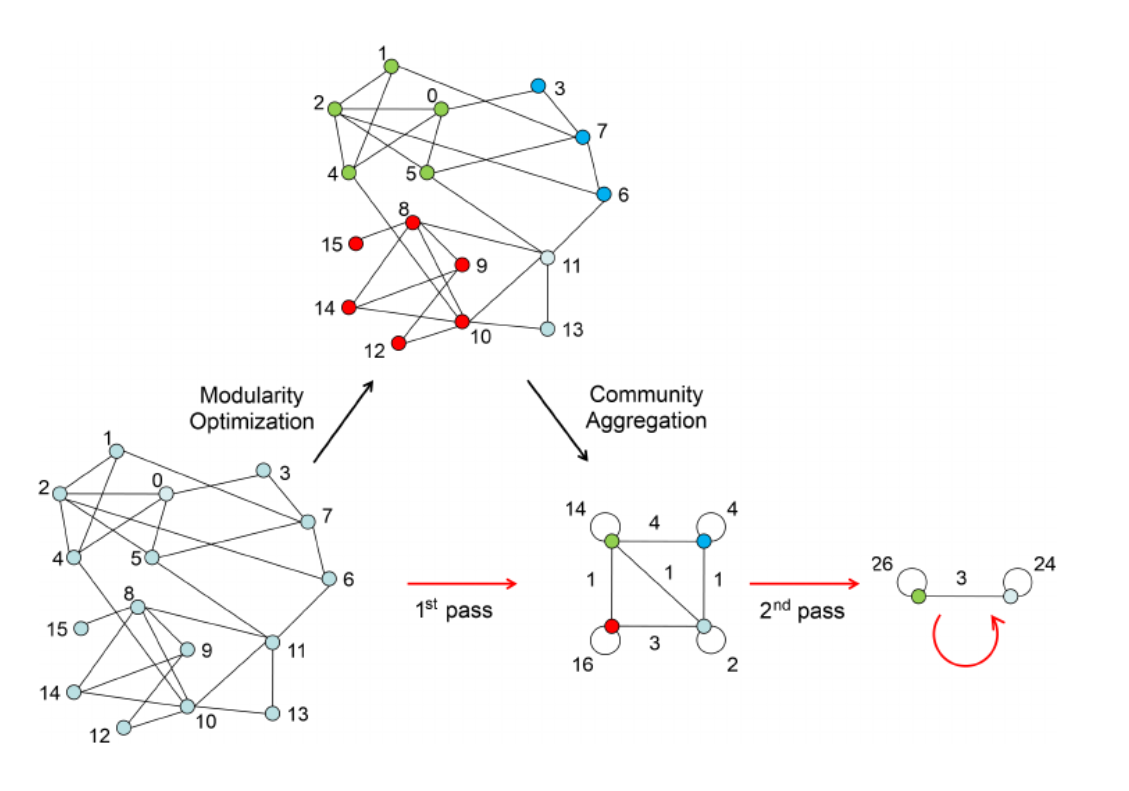
\includegraphics[width=0.7 \textwidth]{Louvain.png}
    \caption{Louvain Algorithm}
    \label{subsection}
\end{figure}
\end{center}
\end{frame}

\begin{frame}[fragile]{PseudoCode}
\resizebox{0.8\textwidth}{!}{%
\begin{algorithm}[H]
    \setcounter{AlgoLine}{0}
    \SetAlgoLined
    \SetKwInOut{Input}{Input}
    \SetKwInOut{Output}{Output}

    \Input{Graph $G$}
    \Output{Communities}

    \BlankLine

    Initialize each node in $G$ as a separate community\;
    
    Initialize the change indicator $modularity_{improvement}$\;

    \Repeat{$\text{modularity\_improvement}$ is not positive}{
        $\text{modularity\_improvement} \gets 0$\;

        \For{each node $i$ in $G$}{
            \For{each neighbor $j$ of node $i$}{
                Merge community of node $i$ with community of node $j$\;
                
                Compute the modularity improvement\;
                
                Undo the merge if the improvement is not positive\;
                
                Track the maximum improvement\;
            }
        }
    }

    \caption{Louvain Algorithm}
\end{algorithm}}
\end{frame}

\begin{frame}[fragile]{Pros and Cons}
Pros:
\begin{itemize}
    \item Fast and scalable for large networks.
    \item Optimizes modularity, which measures community quality.
    \item Detects hierarchical community structures.
    \item Allows flexibility in resolution for different levels of detail.
    \item Widely used with extensive resources and documentation.
\end{itemize}

Cons:
\begin{itemize}
    \item Resolution limit may merge small communities into larger ones.
    \item Results can be sensitive to initial community assignments.
    \item Assumes non-overlapping communities.
    \item Bias towards detecting large, cohesive communities.
    \item Lacks theoretical guarantees of optimality.
\end{itemize}
\end{frame}

\subsection{Label Propagation}
\begin{frame}[fragile]{Intuition}
 The advantage of this algorithm over the other methods is its simplicity and time efficiency. The algorithm uses the network structure to guide its progress and does not optimize any specific chosen measure of community strengths.
\end{frame}

\begin{frame}[fragile]{Pseudocode}
\begin{enumerate}
\item Initialize the labels at all nodes in the network. For a given node $x$, $C_{x}(0) = x$.
\item Initialize $t = 1$.
\item Arrange the nodes in the network in a random order and set it to $X$.
\item For each $x$ in $X$ chosen in that specific order, let $C_{x}(t) = f(C_{x_{i1}}(t),\ldots,C_{x_{im}}(t),C_{x_{i(m+1)}}(t-1),\ldots,C_{x_{ik}}(t-1))$.\\
     $f$ here returns the label occurring with the highest frequency among neighbors and selects a label at random if there are multiple highest-frequency labels.
\item If every node has a label that the maximum number of neighbors have, stop the algorithm. Else, increment $t$ and go to 3.
\end{enumerate}
\end{frame}

\begin{frame}[fragile]{Example}
We have purposely generated a random graph with two evident communities as below. In the first step, we initiated all the nodes with unique labels.
\begin{figure}
\centering
\includegraphics[width=0.5\textwidth]{init_graph.png}
\caption{Combined graph of two sub-graphs.}
\end{figure}
\end{frame}

\begin{frame}[fragile]{Example}
Iteration 1
\begin{itemize}
    \item Node 0 has label 0, has neighbors [2, 3, 7] with labels [2, 3, 7], majority label is 2, so set label of node 0 to 2.
    \item Node 3 has label 3, has neighbors [0, 1, 5, 6] with labels [2, 1, 5, 6], majority label is 1, so set label of node 3 to 1.
    \item Node 6 has label 6, has neighbors [3, 7, 8, 11] with labels [1, 7, 8, 11], majority label is 8, so set label of node 6 to 8.
    \item ...
\end{itemize}
\end{frame}

\begin{frame}[fragile]{Example}
\begin{figure}
\centering
\includegraphics[width=0.65\textwidth]{it_1.png}
\caption{Result at iteration 1.}
\end{figure}
\end{frame}

\begin{frame}[fragile]{Example}
\begin{figure}
\centering
\includegraphics[width=0.65\textwidth]{it_12.png}
\caption{Result at iteration 12.}
\end{figure}
\end{frame}

\begin{frame}[fragile]{Complexity}
\begin{itemize}
    \item Initializing every node with unique labels requires $O(n)$ time.
    \item In each interaction of the label propagation, we first group the neighbors at each node $x$ according to their labels $O(d_{x})$ (degree of a $x$). We then pick the maximum size group and assign its label to $x$, requiring a worst-case time of $O(d_{x})$.
    \item This process is repeated at all nodes; hence, an overall time is $O(m)$ for each iteration based on the assumption that a node's average degree (number of neighbors) is often relatively small compared to the total number of nodes.
\end{itemize}
\end{frame}

\begin{frame}[fragile]{Pros and Cons}
Pros:
\begin{itemize}
    \item Label propagation is computationally efficient, making it suitable for large networks. Its running time is generally faster compared to some other community detection algorithms.
    \item Its noteworthy strength lies in its minimal reliance on prior knowledge of the network structure. There's no need to pre-specify parameters, which proves beneficial when network characteristics are unclear.
\end{itemize}
Cons:
\begin{itemize}
    \item The algorithm doesn't guarantee a unique solution.
\end{itemize}
\end{frame}